\documentclass[../../layout.tex]{subfiles}

\begin{document}
\chapter{Fundamentação teórica}
\hspace*{3em}O estudo, entendimento e compreensão dos conceitos abordados nesse projeto são de suma extema importância para sua compreensão.
do projeto.

\section{Internet das Coisas}
\hspace*{3em}\blindtext[1]
\subsection{Evolução da Internet das Coisas}
\hspace*{3em}\blindtext[1]
\subsection{Internet das Coisas e Indústria 4.0}
\hspace*{3em}\blindtext[1]

\section{Moddelo ultilizado para aplicação}
\hspace*{3em}Para o desenvolvimento da aplicação  utilizamos o modelo cliente servidor em três camadas, esse modelo permite a modularização da aplicação  em três camadas,  camada de interface com usuário, também conhecida como front end, camada lógica onde está inserida as regras de negócio também conhecido como backend e a camada de dados  onde realiza-se a comunicação com o banco de dados, essa arquitetura permite um desacoplamento do código que possibilita a atualização desta partes independente da tecnologia. \cite{3layers}

\section{REST API}

\section{Backend}

\subsection{Conceito de backend}
\hspace*{3em}\blindtext[1]

\subsection{Linguagem Banckend}
\hspace*{3em}A linguagem mais utilizada para programar dispositivos IoT é a linguagem C por ser mais otimizada para essa finalidade, mas por ser uma linguagem de baixo nível, exige uma extensa dedicação de tempo e torna-se moroso para soluções mais complexas. E para contornar essas deficiências a linguagem Elixir pode ser uma ótima alternativa por ser uma linguagem de alto  nível que não compromete tanto a performance do sistema.\par
A linguagem Erlang/Elixir é uma linguagem funcional desenvolvida para atingir alta performance e confiabilidade. Foi desenvolvida para aplicações voltadas para telecomunicações que exigem, baixa tolerancia de falhas, distribuida e real-time (tempo de execução). Por isso conta com um conjunto bibliotecas para desenvolvimento de sistemas de alta confiabilidade conhecida como OTP.\par
Elixir foi desenvolvida para ser executada na VM (máquina virtual) do Erlang nomeada como BEAM. A linguagem Elixir é relativamente nova mas já existem diversas aplicações que a utilizam e inclusive existem recursos para dispositivo embarcado como o caso do framework Nerves.\cite{ElixirorIoT}

\subsection{Nerves}
\hspace*{3em}Nerves é um framework para desenvolvimento de projetos embarcados, baseado em Linux que apenas executa a VM BEAM, portanto proporcionando a utilização da linguagem Elixir para o desenvolvimento das aplicações, dessa forma desfrutando do potencial da linguagem para implementação de projetos embarcados. Além disso este framework proporciona diversas vantagens  em relação ao processo tradicional de programação de embarcados, como, permite a fácil portabilidade para diferentes HW (hardware) embarcados e com uma vasta abrangência para diferentes HW embarcados, fácil manutenção e atualização de firmware por viabilizar a atualizações via OTA (atualização sobre o ar), dispensando o processo tradicional de dispor do acesso físico a flash do dispositivo para o armazenamento do firmware, proporciona também recursos para facilitar e agilizar o desenvolvimento de firmware e uma vasta biblioteca para manipulação dos sistemas embarcados. 

\subsection{Phoenix}
\hspace*{3em}\blindtext[1]


\section{Frontend}
\hspace*{3em}\blindtext[1]

\begin{figure}[H]
\centering
\caption{Diagrama do software}
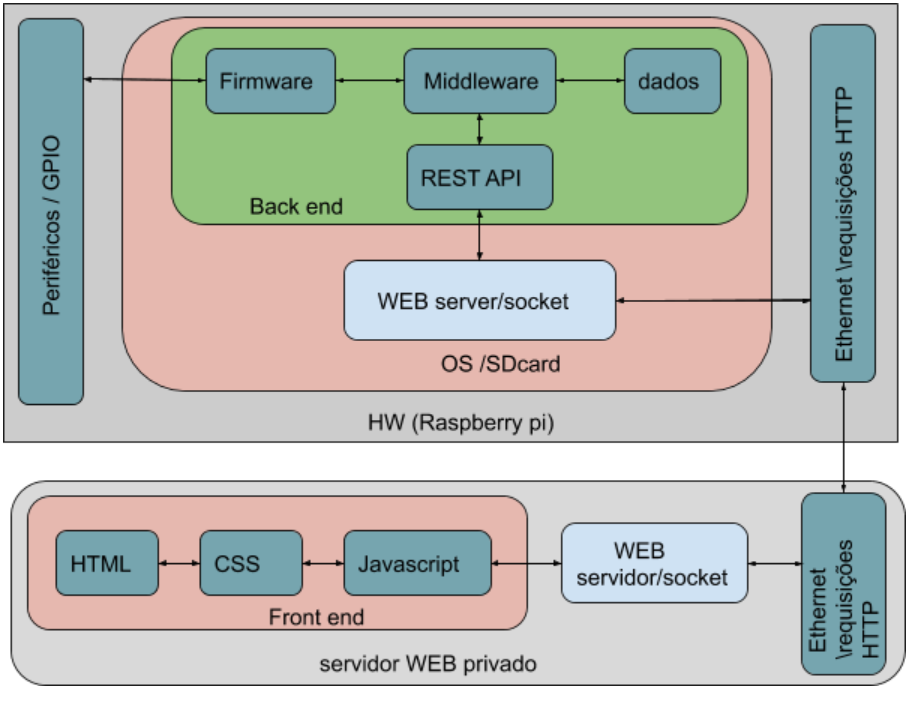
\includegraphics[width=0.5\textwidth]{assets/static/img/diagrama_tcc.PNG}
\label{fig:diagrama_sw}
\end{figure}

\section{Protocolos de comunicação} 
\hspace*{3em}\blindtext[1]
\subsection{i2c}
\hspace*{3em}\blindtext[1]
\subsection{1-wire}
\hspace*{3em}\blindtext[1]
\subsection{UART}
\hspace*{3em}\blindtext[1]

\section{Modelagem do Hardware}
\hspace*{3em}\blindtext[1]

\section{Sensores}
\hspace*{3em}\blindtext[1]

\section{Estrutura do Software}
\hspace*{3em}\blindtext[1]

\section{Método}
\hspace*{3em}\blindtext[1]

\end{document}
